\documentclass[12pt]{article}

\usepackage[utf8]{inputenc}
\usepackage{amsmath, amssymb, amsfonts, cancel}
\usepackage{graphicx}
\usepackage[letterpaper, left=1in, right=1in, top=1in, bottom=1in]{geometry}
\usepackage{booktabs}
\usepackage{multirow}
\usepackage{float}
\usepackage{caption}
\usepackage{colortbl}
\usepackage{xcolor}
\definecolor{paleYellow}{RGB}{255,255,180}
\usepackage{physics}
\usepackage{hyperref}
\usepackage[spanish]{babel}
\usepackage{setspace}
\usepackage{listings}
\usepackage{xcolor}


\lstset{
    backgroundcolor=\color{gray!10},
    basicstyle=\ttfamily,
    breaklines=true,
    frame=single
}

\title{
Práctica 9: Seguridad del puerto\\[0.5em]
\large Administración de redes
}

\author{
Jorge Alberto Suarez Saldana\\
\small Matrícula: 355992\\
\small Profesor: Raymundo Antonio González Grimaldo
}

\date{\today}

\begin{document}
\maketitle

\section{Objetivo}
Configurar y verificar la seguridad de puertos en un switch para restringir el acceso a dispositivos autorizados mediante direcciones MAC.

\section{Desarrollo}

\subsection{Paso 1: Configuración de la seguridad del puerto}

Se accedió al switch S1 y se habilitó la seguridad en los puertos FastEthernet 0/1 y 0/2:

\begin{lstlisting}
S1(config)# interface range f0/1 - 2
S1(config-if-range)# switchport port-security
\end{lstlisting}

Se configuró el máximo de dispositivos permitidos por puerto:

\begin{lstlisting}
S1(config-if-range)# switchport port-security maximum 1
\end{lstlisting}

Se habilitó el aprendizaje dinámico de direcciones MAC (sticky):

\begin{lstlisting}
S1(config-if-range)# switchport port-security mac-address sticky
\end{lstlisting}

Se configuró el modo de violación como \textit{restrict}:

\begin{lstlisting}
S1(config-if-range)# switchport port-security violation restrict
\end{lstlisting}

Finalmente, se deshabilitaron los puertos no utilizados:

\begin{lstlisting}
S1(config)# interface range f0/3 - 24 , g0/1 - 2
S1(config-if-range)# shutdown
\end{lstlisting}

\subsection{Paso 2: Verificación}

Se comprobó la conectividad entre PC1 y PC2 mediante \textit{ping}, obteniendo resultados exitosos.

Se verificó la configuración activa:

\begin{lstlisting}
S1# show run | begin interface
S1# show port-security
S1# show port-security address
\end{lstlisting}

Las direcciones MAC de PC1 y PC2 fueron aprendidas correctamente mediante el método \textit{sticky}.

Posteriormente, se conectó una laptop intrusa a un puerto del switch, observando indicadores de violación (LED rojo).

Al habilitar el puerto, la laptop pudo comunicarse temporalmente. Sin embargo, al conectarla al puerto F0/2 (originalmente usado por PC2), no logró establecer comunicación con PC1.

Se verificaron las violaciones con:

\begin{lstlisting}
S1# show port-security interface f0/2
\end{lstlisting}

\section{Resultados}

\subsection{Pregunta 1}
\textbf{¿Cuántas violaciones han ocurrido?}

Se registró al menos una violación de seguridad al intentar conectar un dispositivo no autorizado en un puerto con MAC previamente aprendida.

\subsection{Pregunta 2}
\textbf{¿Por qué la PC2 puede hacer ping a PC1, pero la laptop intrusa no?}

Porque la dirección MAC de PC2 fue aprendida y almacenada mediante el mecanismo \textit{sticky}, quedando registrada como dispositivo autorizado en el puerto. 

En cambio, la laptop intrusa posee una dirección MAC distinta, la cual no coincide con la configurada en el puerto. Debido a la política de seguridad (\textit{maximum 1} y modo \textit{restrict}), el switch bloquea el tráfico proveniente de direcciones no autorizadas, impidiendo la comunicación.

\subsection{Capturas de pantalla}
\begin{figure}[H]
  \centering
  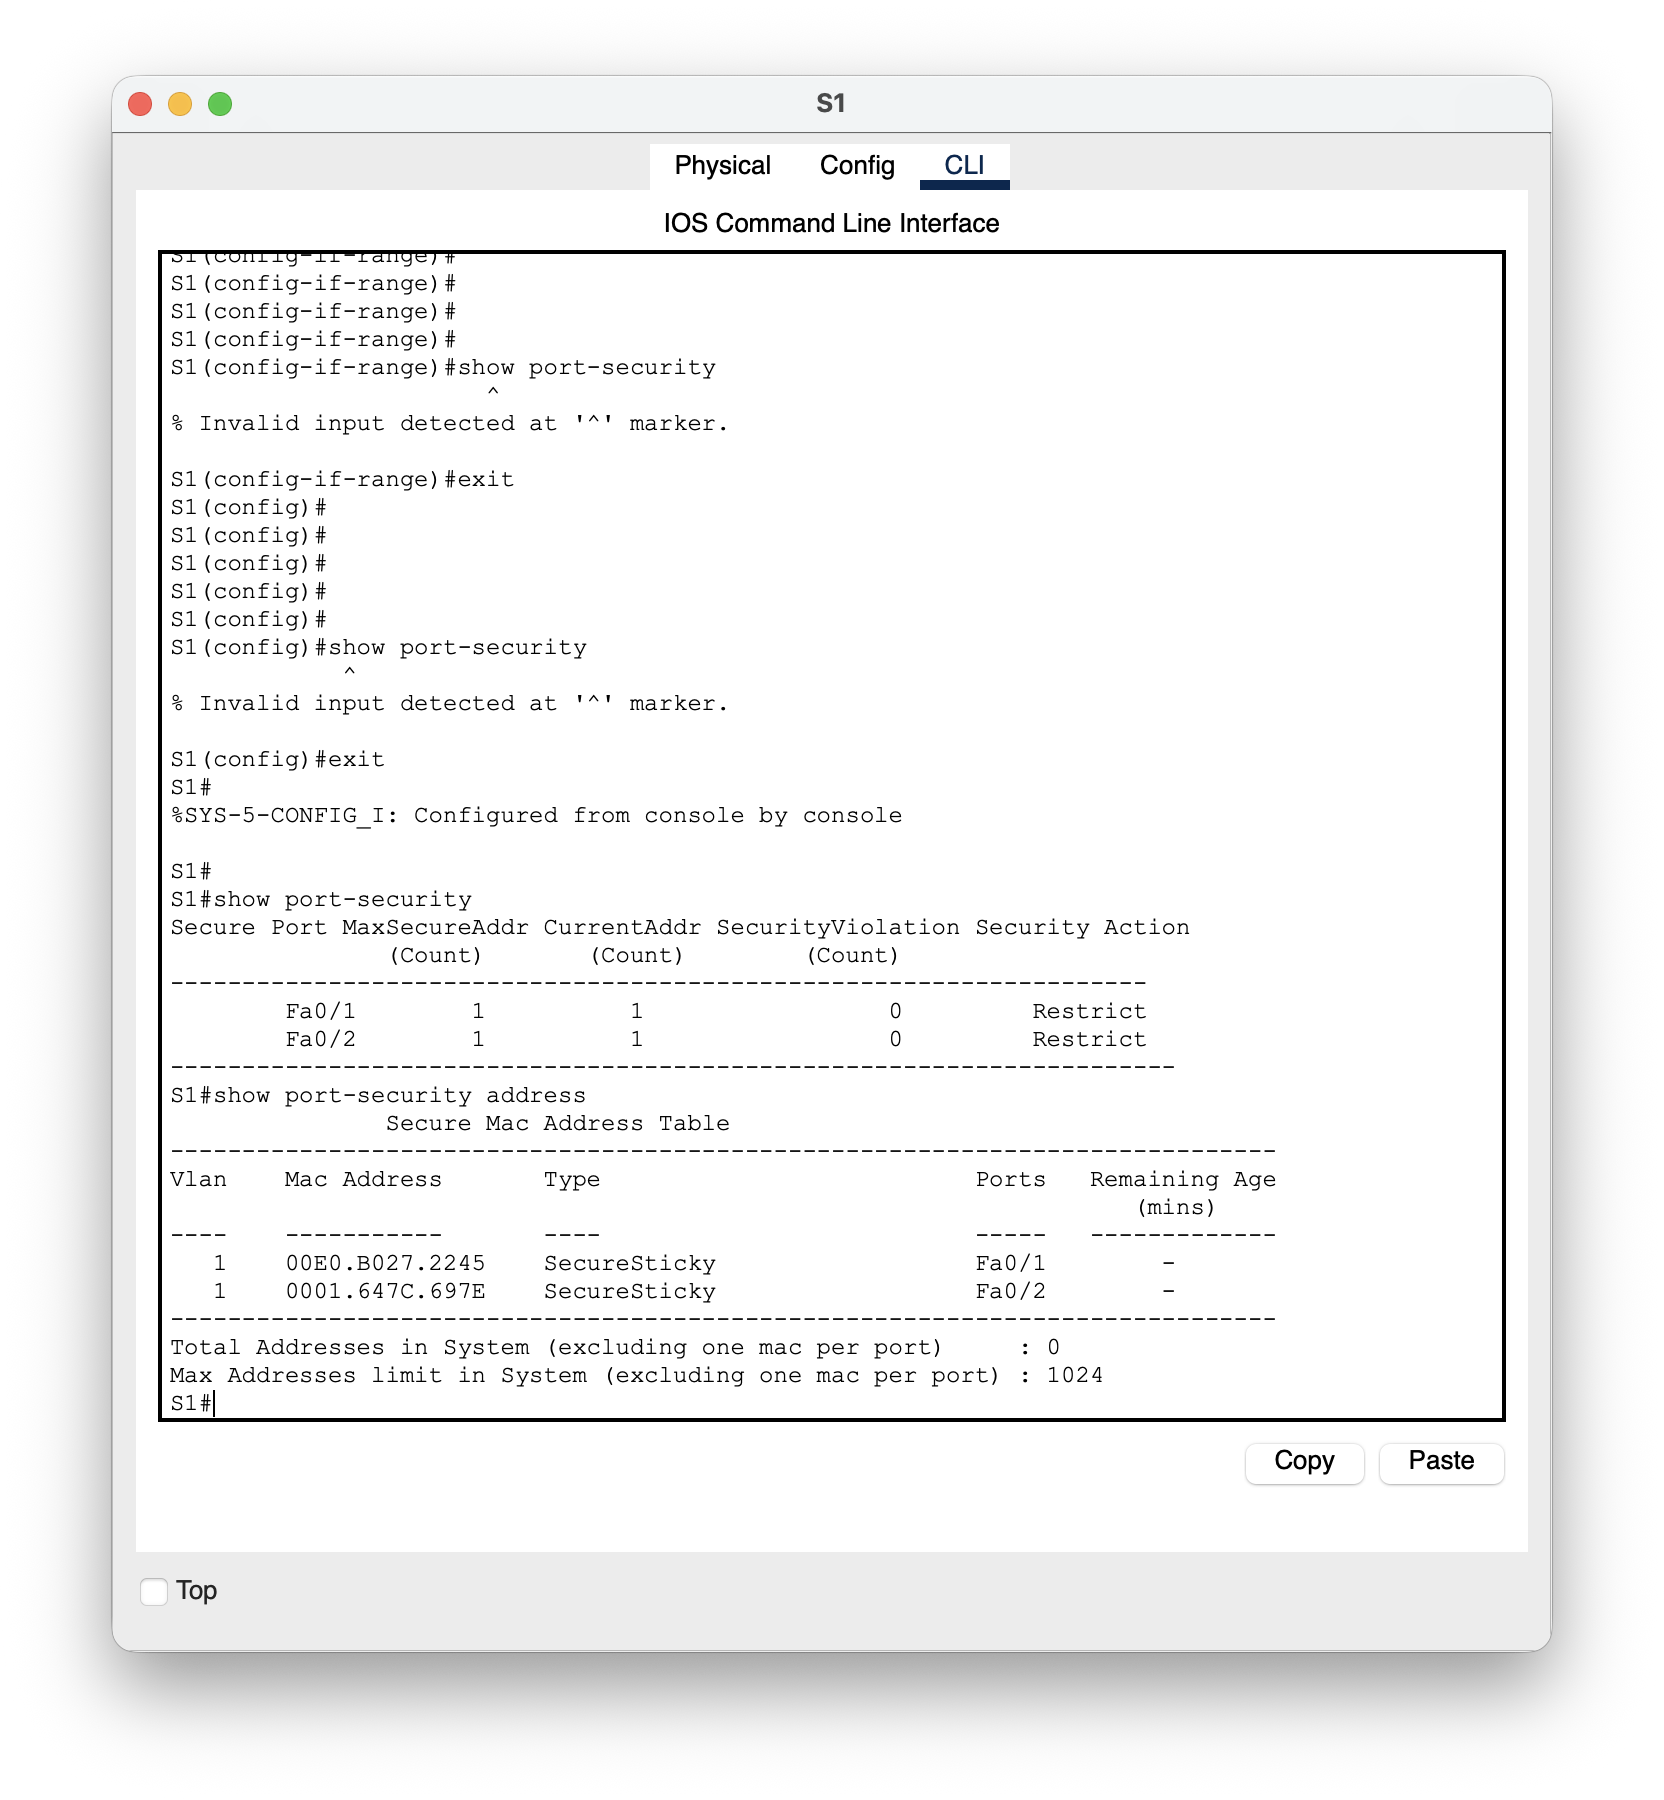
\includegraphics[width=0.8\textwidth]{salidasComandos.png}
  \caption{Salida de los comandos show port-security y show port-security address}\label{fig:salidasComandos}
\end{figure}

\begin{figure}[H]
  \centering
  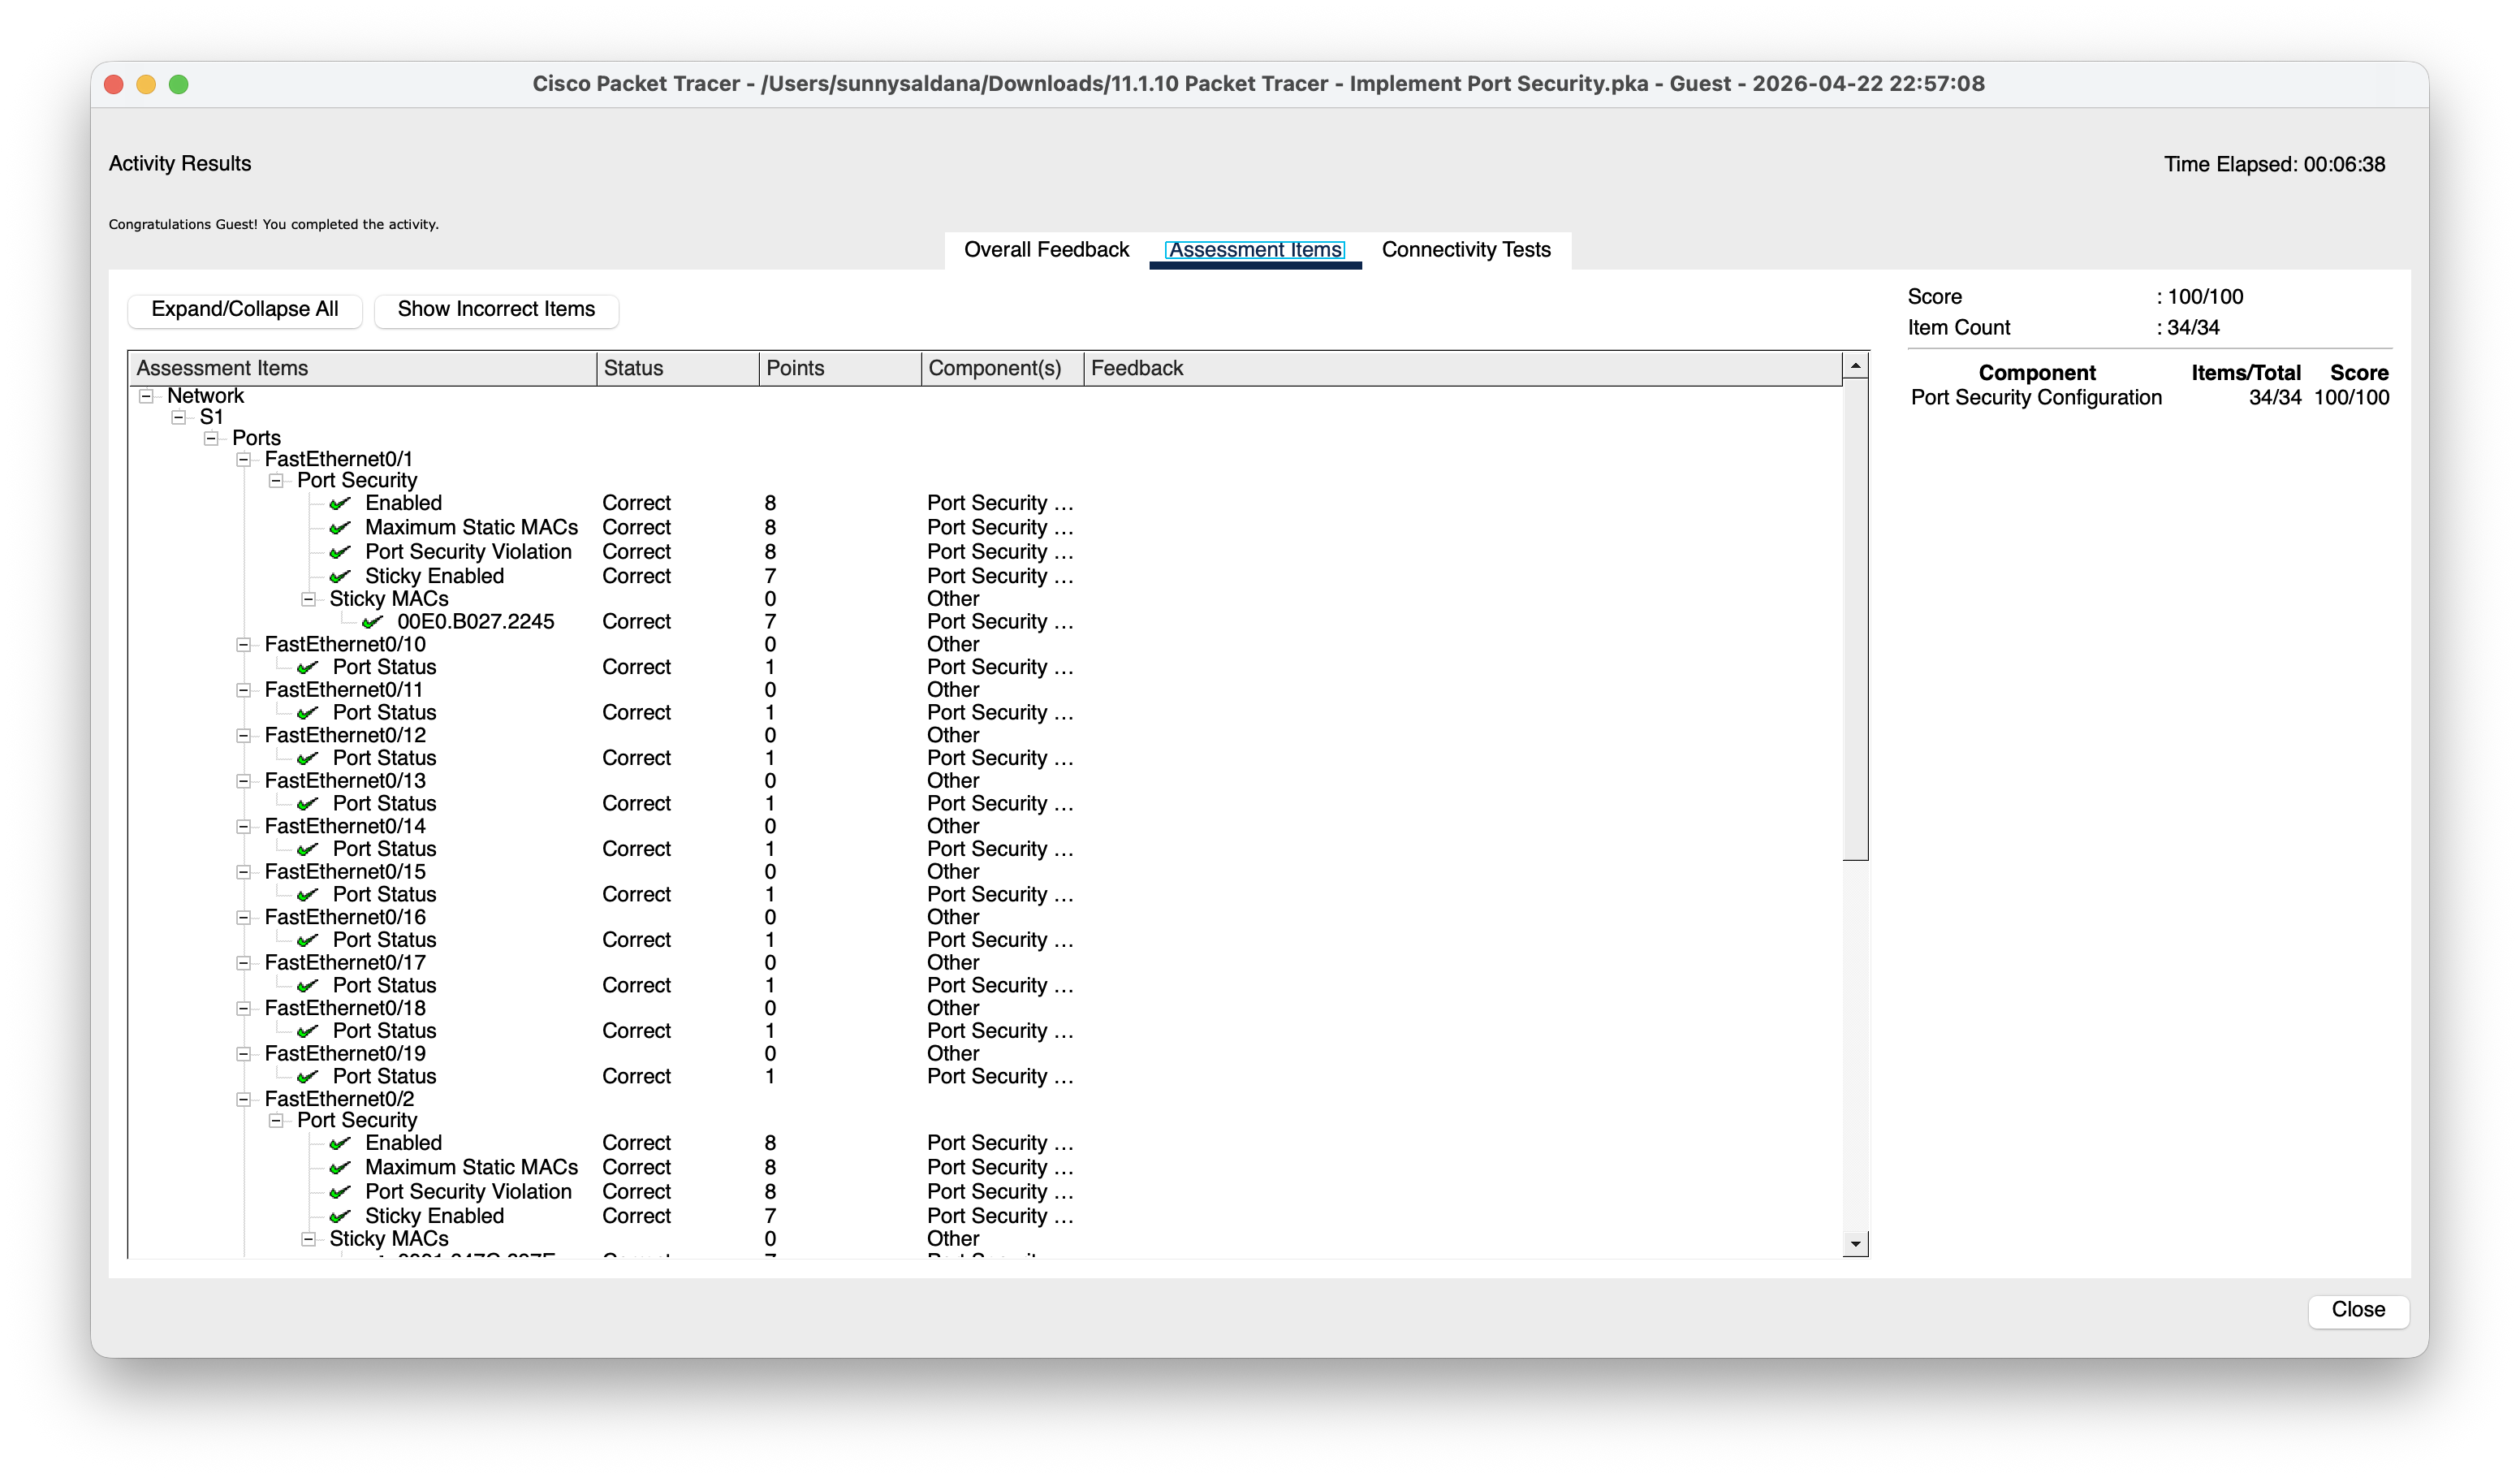
\includegraphics[width=0.8\textwidth]{resultadosCheck.png}
  \caption{Resultados Packet Tracer}\label{fig:resultadosCheck}
\end{figure}

\section{Conclusión}

La seguridad de puertos permite controlar el acceso a la red a nivel de capa 2, limitando los dispositivos permitidos por interfaz. El uso de direcciones MAC sticky facilita la administración al aprender automáticamente dispositivos válidos. 

El modo de violación \textit{restrict} resulta útil ya que evita deshabilitar el puerto, pero bloquea tráfico no autorizado y registra los intentos de acceso indebido.

\end{document}